\documentclass[12pt]{article}
\usepackage{amsmath, amsthm, amssymb}
\usepackage{hyperref}
\usepackage[margin=1cm]{caption}
\usepackage{verbatim}
\usepackage[top=1.0in, bottom=1.0in, left=1.0in, right=1.0in]{geometry}
\usepackage{graphicx}

\pagestyle{plain}

\usepackage{tkz-graph}
\usetikzlibrary{arrows}
\usetikzlibrary{shapes}
\usepackage[position=bottom]{subfig}

\usepackage{longtable}
\usepackage{array}

\usepackage{sectsty}
\allsectionsfont{\sffamily}

\setcounter{secnumdepth}{5}
\setcounter{tocdepth}{5}

\makeatletter
\newtheorem*{rep@theorem}{\rep@title}
\newcommand{\newreptheorem}[2]{
\newenvironment{rep#1}[1]{
 \def\rep@title{#2 \ref{##1}}
 \begin{rep@theorem}}
 {\end{rep@theorem}}}
\makeatother

\theoremstyle{plain}
\newtheorem{thm}{Theorem}[section]
\newreptheorem{thm}{Theorem}
\newtheorem{prop}[thm]{Proposition}
\newreptheorem{prop}{Proposition}
\newtheorem{lem}[thm]{Lemma}
\newreptheorem{lem}{Lemma}
\newtheorem{conjecture}[thm]{Conjecture}
\newreptheorem{conjecture}{Conjecture}
\newtheorem{cor}[thm]{Corollary}
\newreptheorem{cor}{Corollary}
\newtheorem{prob}[thm]{Problem}
\newtheorem{observation}{Observation}
\newtheorem{obs}[observation]{Observation}
\newtheorem*{mainconj}{Main Conjecture}
\newtheorem*{mainthm}{Main Theorem}
\newtheorem{problem}{Problem}
\newtheorem{clm}{Claim}

\theoremstyle{definition}
\newtheorem{defn}{Definition}
\theoremstyle{remark}
\newtheorem*{remark}{Remark}
\newtheorem{example}{Example}
\newtheorem*{question}{Question}


\newcommand{\fancy}[1]{\mathcal{#1}}
\newcommand{\C}[1]{\fancy{C}_{#1}}
\newcommand{\IN}{\mathbb{N}}
\newcommand{\IR}{\mathbb{R}}
\newcommand{\G}{\fancy{G}}
\newcommand{\CC}{\fancy{C}}
\newcommand{\D}{\fancy{D}}

\newcommand{\inj}{\hookrightarrow}
\newcommand{\surj}{\twoheadrightarrow}

\newcommand{\set}[1]{\left\{ #1 \right\}}
\newcommand{\setb}[3]{\left\{ #1 \in #2 \mid #3 \right\}}
\newcommand{\setbs}[2]{\left\{ #1 \mid #2 \right\}}
\newcommand{\card}[1]{\left|#1\right|}
\newcommand{\size}[1]{\left\Vert#1\right\Vert}
\newcommand{\ceil}[1]{\left\lceil#1\right\rceil}
\newcommand{\floor}[1]{\left\lfloor#1\right\rfloor}
\newcommand{\func}[3]{#1\colon #2 \rightarrow #3}
\newcommand{\funcinj}[3]{#1\colon #2 \inj #3}
\newcommand{\funcsurj}[3]{#1\colon #2 \surj #3}
\newcommand{\irange}[1]{\left[#1\right]}
\newcommand{\join}[2]{#1 \mbox{\hspace{2 pt}$\ast$\hspace{2 pt}} #2}
\newcommand{\djunion}[2]{#1 \mbox{\hspace{2 pt}$+$\hspace{2 pt}} #2}
\newcommand{\parens}[1]{\left( #1 \right)}
\newcommand{\brackets}[1]{\left[ #1 \right]}
\newcommand{\nint}[1]{\widetilde{N}\left(#1\right)}
\newcommand{\DefinedAs}{\mathrel{\mathop:}=}
\newcommand{\pot}{\operatorname{pot}}

\def\adj{\leftrightarrow}
\def\nonadj{\not\!\leftrightarrow}

\def\D{\fancy{D}}
\def\C{\fancy{C}}
\def\Q{\fancy{Q}}
\def\Z{\fancy{Z}}
\def\H{\fancy{H}}
\def\L{\fancy{L}}
\def\B{\fancy{B}}

% any changes to \claim should be mirrored in \claimnonum and \subclaim
\newcommand{\claim}[2]{{\bf Claim #1.}~{\it #2}~~}
\newcommand{\claimnonum}[1]{{\bf Claim.}~{\it #1}~~}
\newcommand{\subclaim}[2]{{\bf Subclaim #1.}~{\it #2}~~}

\newcommand\numberthis{\addtocounter{equation}{1}\tag{\theequation}}

%
%  If the proof ends with a displayed equation, use \aftermath just
%  before \end{proof} to put the halmos in the ``right'' place.  This
%  may not work near page boundaries. 
%
\def\aftermath{\par\vspace{-\belowdisplayskip}\vspace{-\parskip}\vspace{-\baselineskip}}

\def\fr{\frac}
\def\adj{\leftrightarrow}
\def\ch{\textrm{ch}}

\renewcommand{\restriction}{\mathord{\upharpoonright}}
\begin{document}
\title{most low Alon-Tarsi notes}
\author{}
\maketitle

\section{Introduction}

We consider graphs with vertices labeled by natural numbers; that is, pairs $(G,h)$ where $G$ is a graph and $\func{h}{V(G)}{\IN}$.  We say that \emph{$(G, h)$ is AT} if $G$ is $(d_G - h)$-AT.

\section{Subgraphs, subdivisions and cuts}
\begin{defn}
	A graph $G$ is \emph{$h$-minimal} if $G$ is connected and $\parens{H, h\restriction_{V(H)}}$ is not AT for every proper induced subgraph $H$ of $G$ where $h(v) = 0$ for all $v \in V(G) \setminus V(H)$.	
\end{defn}

\begin{lem}\label{InducedSubgraph}
	If $G$ is connected and $(G,h)$ is not AT, then $G$ is $h$-minimal.
\end{lem}
\begin{proof}
	If there were a proper induced subgraph $H$ such that $\parens{H, h\restriction_{V(H)}}$ is AT, then by ordering the vertices of each component of $G - V(H)$ by increasing distance to $H$ and directing all edges away from $H$ in this order we conclude that $(G,h)$ is AT.
\end{proof}

\begin{lem}\label{SubdivideTwice}
	If $(G',h')$ is formed from $(G,h)$ by subdividing an edge $e$ of $G$ twice and having $h'$ give zero on the two new vertices, then
	\begin{enumerate}
		\item if $(G,h)$ is AT, then $(G', h')$ is AT; and
		\item if $(G', h')$ is AT, then either $(G,h)$ is AT or $(G-e,h)$ is AT.
	\end{enumerate}	
\end{lem}
\begin{proof}
	Suppose $e = xy$ and call the new vertices $x'$ and $y'$ so that $G'$ contains the induced path $xx'y'y$.	For (1), let $D$ be an orientation of $G$ showing that $(G,h)$ is AT. By symmetry we may assume $xy \in E(D)$. Make an orientation $D'$ of $G'$ from $D$ by replacing $xy$ with the directed path $xx'y'y$.  There is a natural parity preserving bijection between the spanning Eulerian subgraphs of $D$ and $D'$, so we conclude that $(G', h')$ is AT.
	
	For (2), let $D'$ be an orientation of $G'$ showing that $(G',h')$ is AT.  Suppose $G'$ contains the directed path $xx'y'y$ or the directed path $yy'x'x$.  By symmetry, we can assume it is $xx'y'y$.  Then make an orientation $D$ of $G$ by replacing $xx'y'y$ with the directed edge $xy$.  As above, we have a parity preserving bijection between the spanning Eulerian subgraphs of $D$ and $D'$, so we conclude that $(G, h)$ is AT.  Otherwise, no spanning Eulerian subgraph of $D'$ contains a cycle passing through $x'$ and $y'$.  So, the spanning Eulerian subgraph counts of $D'$ are the same as those of $D' - x' - y'$.  But this gives an orientation of $G-e$ showing that $(G-e, h)$ is AT.
\end{proof}

\begin{cor}\label{ReduceP4Cor}
	Let $G$ be an $h$-minimal graph.  If $(G,h)$ is AT and $G$ has an induced path $x_1x_2x_3x_4$ such that $d_G(x_2) = d_G(x_3) = 2$ and $h(x_2) = h(x_3) = 0$, then 
	\[\parens{(G - x_2 - x_3) + x_1x_4, h\restriction_{V(G) \setminus \set{x_2, x_3}}} \text{ is AT.}\]
\end{cor}
\begin{proof}
	Suppose $(G,h)$ is AT and $G$ has such an induced path $x_1x_2x_3x_4$.  Applying Lemma \ref{SubdivideTwice} part (2) shows that either $\parens{G - x_2 - x_3, h\restriction_{V(G) \setminus \set{x_2, x_3}}}$ is AT or $\parens{(G - x_2 - x_3) + x_1x_4, h\restriction_{V(G) \setminus \set{x_2, x_3}}}$ is AT.  But $G - x_2 - x_3$ is a proper induced subgraph of $G$, so the former cannot happen since $G$ is $h$-minimal and $h(x_2) = h(x_3) = 0$.  Hence $\parens{(G - x_2 - x_3) + x_1x_4, h\restriction_{V(G) \setminus \set{x_2, x_3}}}$ is AT.
\end{proof}

\begin{lem}\label{CutvertexPatch}
	Let $\set{A_1, A_2}$ be a separation of $G$ such that $A_1 \cap A_2 = \set{x}$.  If $G[A_i]$ is $f_i$-AT for $i \in \irange{2}$, then $G$ is $f$-AT where $f(v) = f_i(v)$ for $v \in V(A_i-x)$ and $f(x) = f_1(x) + f_2(x) - 1$.  Going the other direction, if $G$ is $f$-AT, then $G[A_i]$ is $f_i$-AT for $i \in \irange{2}$ where $f_i(v) = f(v)$ for $v \in V(A_i-x)$ and $f_1(x) + f_2(x) \le f(x) + 1$.
\end{lem}
\begin{proof}
	For $i \in \irange{2}$, choose an orientation $D_i$ of $A_i$ showing that $A_i$ is $f_i$-AT.  Together these give an orientation $D$ of $G$ and since no cycle has vertices in both $A_1-x$ and $A_2-x$, we have
	\begin{align*}
		EE(D) - EO(D) &= EE(D_1)EE(D_2) + EO(D_1)EO(D_2) - (EE(D_1)EO(D_2) + EO(D_1)EE(D_2)) \\
		&= (EE(D_1) - EO(D_1))(EE(D_2) - EO(D_2)) \\
		&\ne 0.
	\end{align*}
	Hence $G$ is $f$-AT.
	
	Now, suppose $G$ is $f$-AT and choose an orientation $D$ of $G$ showing this.  Put $D_i = D[A_i]$ for $i \in \irange{2}$.  Then, as above, we have $0 \ne EE(D) - EO(D) = (EE(D_1) - EO(D_1))(EE(D_2) - EO(D_2))$ and hence $EE(D_1) - EO(D_1) \ne 0$ and $EE(D_2) - EO(D_2) \ne 0$.  Since the in-degree of $x$ in $D$ is the sum of the in-degree of $x$ in $D_1$ and the in-degree of $x$ in $D_2$, the lemma follows.
\end{proof}

\section{Extension lemma}
This is a key lemma from \cite{OreVizing}, it generalizes a lemma from \cite{kostochkastiebitzedgesincriticalgraph} from list coloring to Alon-Tarsi orientations.  
This is what i talked about in Baltimore.  The basic idea is that in some cases we can pair off odd/even spanning Eulerian subgraphs via a parity reversing bijection.

\begin{lem}\label{GeneralEulerLemma}
	Let $G$ be a multigraph without loops and $\func{f}{V(G)}{\IN}$. If there are $F \subseteq G$ and
	$Y \subseteq V(G)$ such that:
	\begin{enumerate}
		\item any multiple edges in $G$ are contained in $G[Y]$; and
		\item $f(v) \ge d_G(v)$ for all $v \in V(G) \setminus Y$; and
		\item $f(v) \ge d_{G[Y]}(v) + d_F(v) + 1$ for all $v \in Y$; and
		\item For each component $T$ of $G-Y$ there are different $x_1, x_2 \in V(T)$ where $N_T[x_1] = N_T[x_2]$ and $T - \set{x_1, x_2}$ is connected such that either:
		\begin{enumerate}
			\item there are $x_1y_1, x_2y_2 \in E(F)$ where $y_1 \ne y_2$ and $N(x_i) \cap Y = \set{y_i}$ for $i \in \irange{2}$; or
			\item $\card{N(x_2) \cap Y} = 0$ and there is $x_1y_1 \in E(F)$ where $N(x_1) \cap Y = \set{y_1}$,
		\end{enumerate}
	\end{enumerate}
	
	\noindent then $G$ is $f$-AT.
\end{lem}
\begin{proof}
	Suppose not and pick a counterexample $\parens{G, f, F, Y}$ minimizing $\card{G-Y}$. %HK Changed sentence to fix the typesetting
	If $\card{G-Y} = 0$, then $Y = V(G)$ and thus $f(v) \ge d_G(v) + 1$ for all $v \in V(G)$ by (3).  Pick an acyclic orientation $D$ of $G$.  Then $EE(D) = 1$, $EO(D) = 0$ and $d_D^+(v) \le d_G(v) \le f(v) - 1$ for all $v \in V(D)$. Hence $G$ is $f$-AT.  So, we must have $\card{G-Y} > 0$.  
	
	Pick a component $T$ of $G - Y$ and pick $x_1, x_2 \in V(T)$ as guaranteed by (4). First, suppose (4a) holds.   Put $G' \DefinedAs (G - T) + y_1y_2$, $F' \DefinedAs F - T$, $Y' \DefinedAs Y$ and let $f'$ be $f$ restricted to $V(G')$.  Then $G'$ has an orientation $D'$ where $f'(v) \ge d_{D'}^+(v) + 1$ for all $v \in V(D')$ and $EE(D') \ne EO(D')$, for otherwise $\parens{G', f', F', Y'}$ would contradict minimality.  By symmetry we may assume that the new edge $y_1y_2$ is directed toward $y_2$.  Now we use the orientation of $D'$ to construct the desired orientation of $D$. First, we use the orientation on $D' - y_1y_2$ on $G-T$. Now, order the vertices of $T$ as $x_1, x_2, z_1, z_2, \ldots$ so that every vertex has at least one neighbor to the right.  Orient the edges of $T$ left-to-right in this ordering.  Finally, we use $y_1x_1$ and $x_2y_2$ and orient all other edges between $T$ and $G-T$ away from $T$.  Plainly, $f(v) \ge d_{D}^+(v) + 1$ for all $v \in V(D)$.  Since $y_1x_1$ is the only edge of $D$ going into $T$, any Eulerian subgraph of $D$ that contains a vertex of $T$ must contain $y_1x_1$.  So, any Eulerian subgraph of $D$ either contains (i) neither $y_1x_1$ nor $x_2y_2$, (ii) both $y_1x_1$ and $x_2y_2$, or (iii) $y_1x_1$ but not $x_2y_2$.  We first handle (i) and (ii) together.  Consider the function $h$ that maps an Eulerian subgraph $Q$ of $D'$ to an Eulerian subgraph $h(Q)$ of $D$ as follows.  If $Q$ does not contain $y_1y_2$, let $h(Q) = \iota(Q)$ where $\iota(Q)$ is the natural embedding of $D' - y_1y_2$ in $D$.  Otherwise, let $h(Q) = \iota(Q - y_1y_2) + \set{y_1x_1, x_1x_2, x_2y_2}$.  Then $h$ is a parity-preserving injection with image precisely the union of those Eulerian subgraphs of $D$ in (i) and (ii).  Hence if we can show that exactly half of the Eulerian subgraphs of $D$ in (iii) are even, we will conclude $EE(D) \ne EO(D)$, a contradiction.  To do so, consider an Eulerian subgraph $A$ of $D$ containing $y_1x_1$ and not $x_2y_2$. Since $x_1$ must have in-degree $1$ in $A$, it must also have out-degree $1$ in $A$.  We show that $A$ has a mate $A'$ of opposite parity.  Suppose $x_2 \not \in A$ and $x_1z_1 \in A$; then we make $A'$ by removing $x_1z_1$ from $A$ and adding $x_1x_2z_1$.  If $x_2 \in A$ and $x_1x_2z_1 \in A$, we make $A'$ by removing $x_1x_2z_1$ and adding $x_1z_1$. Hence exactly half of the Eulerian subgraphs of $D$ in (iii) are even and we conclude $EE(D) \ne EO(D)$, a contradiction.
	
	Now suppose (4b) holds.  Put $G' \DefinedAs G - T$, $F' \DefinedAs F - T$, $Y' \DefinedAs Y$ and define $f'$ by $f'(v) = f(v)$ for all $v \in V(G'-y_1)$ and $f'(y_1) = f(y_1) - 1$.  Then $G'$ has an orientation $D'$ where $f'(v) \ge d_{D'}^+(v) + 1$ for all $v \in V(D')$ and $EE(D') \ne EO(D')$, for otherwise $\parens{G', f', F', Y'}$ would contradict minimality.  We orient $G - T$ according to $D$, orient $T$ as in the previous case, again use $y_1x_1$ and orient all other edges between $T$ and $G-T$ away from $T$.  Since we decreased $f'(y_1)$ by $1$, the extra out edge of $y_1$ is accounted for and we have $f(v) \ge d_{D}^+(v) + 1$ for all $v \in V(D)$.  Again any additional Eulerian subgraph must contain $y_1x_1$ and since $x_2$ has no neighbor in $G-T$ we can use $x_2$ as before to build a mate of opposite parity for any additional Eulerian subgraph.  Hence $EE(D) \ne EO(D)$ giving our final contradiction.
\end{proof}

\section{Degree-AT graphs}
A graph $G$ is called \emph{degree-AT} if $(G,h)$ is $AT$ where $h$ is the constant zero function.

\begin{lem}\label{DegreeATClassification}
	A connected graph $G$ is degree-AT if it is not a Gallai tree.
\end{lem}
\begin{proof}
	Suppose there exists a connected graph that is not a Gallai tree, but is also not
	degree-AT.  Let $G$ be such a graph with as few vertices as possible.
	Since $G$ is not degree-AT, no induced subgraph $H$ of $G$ is
	degree-AT by Lemma \ref{InducedSubgraph}. 
	Hence, for any $v \in V(G)$ that is not a cutvertex, $G-v$ must be a Gallai
	tree by minimality of $|G|$.  
	
	If $G$ has more than one block, then for endblocks $B_1$ and $B_2$, choose
	noncutvertices $w\in B_1$ and $x\in B_2$.  By the minimality of $|G|$, both
	$G-w$ and $G-x$ are Gallai trees.  Since every block of $G$ appears either as a
	block of $G-w$ or as a block of $G-x$, every block of $G$ is either complete or
	an odd cycle.  Hence, $G$ is a Gallai tree, a contradiction.  So instead $G$
	has only one block, that is, $G$ is $2$-connected.  Further, $G-v$ is a Gallai
	tree for all $v \in V(G)$.
	
	Let $v$ be a vertex of minimum degree in $G$.  Since $G$ is $2$-connected, $d_G(v) \ge 2$. By Lemma \ref{CutvertexPatch}, $v$ is adjacent to a noncutvertex in every endblock of $G-v$.
	If $G-v$ has a complete block $B$ with noncutvertices $x_1,x_2$ where $v \adj x_1$ and $v \nonadj x_2$, then we can apply Lemma \ref{GeneralEulerLemma} with $Y = \set{v}$ and $F = vx_1$ to conclude that $G$ is degree-AT, a contradiction.  So, $v$ must be adjacent to every noncutvertex in every complete endblock of $G-v$.
	
	Suppose $d_G(v) \ge 3$.  Then no endblock of $G-v$ can be an odd cycle of length at least $5$ (there would be vertices of degree $3$ but we'd have $d_G(v) \ge 4$).  Let $B$ be a smallest complete endblock of $G-v$.  Then for a noncutvertex $x \in V(B)$, we have $d_G(x) = |B|$ and hence $d_G(v) \le |B|$.  If $G-v$ has at least two endblocks, then $2(|B|-1) \le |B|$ and hence $d_G(v) \le |B| = 2$, a contradiction.  Hence $G-v = B$ and $v$ is joined to $B$, so $G$ is complete, a contradiction.
	
	Hence, we must have $d_G(v) = 2$.  Suppose $G-v$ has at least $2$ endblocks.  Then, it has exactly $2$ and $v$ is adjacent to one noncutvertex in each.  Neither of the endblocks can be odd cycles of length at least $5$ since then we could get a smaller counterexample by Lemma \ref{SubdivideTwice}.  Since $v$ is adjacent to every noncutvertex in every complete endblock of $G-v$, both endblocks must be $K_2$.  But then either $G=C_4$ (which is trivially degree-AT) or we can get a smaller counterexample by Lemma \ref{SubdivideTwice}.  So, $G-v$ must be $2$-connected. Since $G-v$ is a Gallai tree, it is either complete or an odd cycle.  If $G-v$ is not complete, we can get a smaller counterexample by Lemma \ref{SubdivideTwice}.  So, $G-v$ is complete and $v$ is adjacent to every noncutvertex of $G-v$; that is, $G$ is complete, a contradiction.
\end{proof}

\section{When h is 1 for at most one vertex}
Here we classify the graphs $G$ such that $(G,h)$ is AT where $\sum_{v \in V(G)} h(v) \le 1$. 

\begin{lem}\label{DegreeTwoVertex}
	Let $G$ be a connected graph and $x \in V(G)$ with $d_G(x) = 2$.  If $h(x) = 1$ and $h(v) = 0$ for all $v \in V(G-x)$, then $(G,h)$ is AT if and only if $G-x$ is degree-AT.
\end{lem}
\begin{proof}
	Let $D$ be an orientation of $G$ showing that $(G,h)$ is AT.  Then $d_{D}^-(x) = 2$ and hence no spanning Eulerian subgraph contains a cycle passing through $x$.  Therefore, the Eulerian subgraph counts in $G-x$ are different and $G-x$ is degree-AT.
	The other direction is immediate from Lemma \ref{InducedSubgraph}.
\end{proof}

\begin{figure}[!htb]
	\centering
	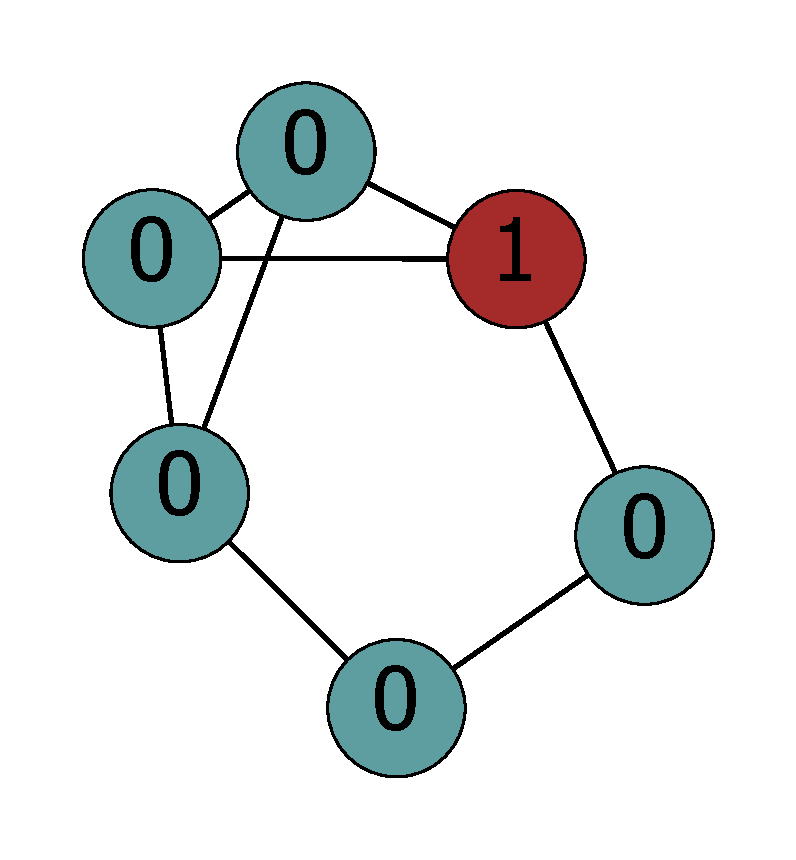
\includegraphics[scale=0.35]{pictures/011010111010010[0,1,0,0,0,0].pdf}
	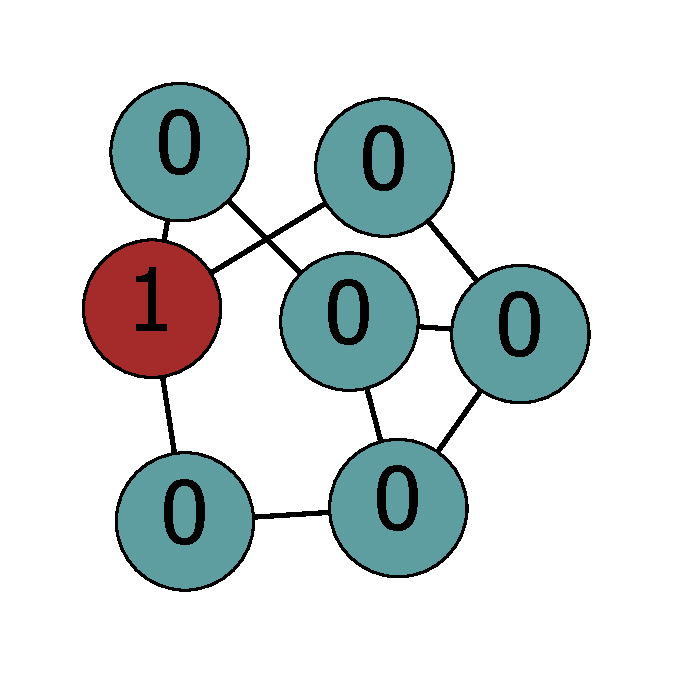
\includegraphics[scale=0.35]{pictures/001101001100011010010[0,0,0,0,0,1,0].pdf}
	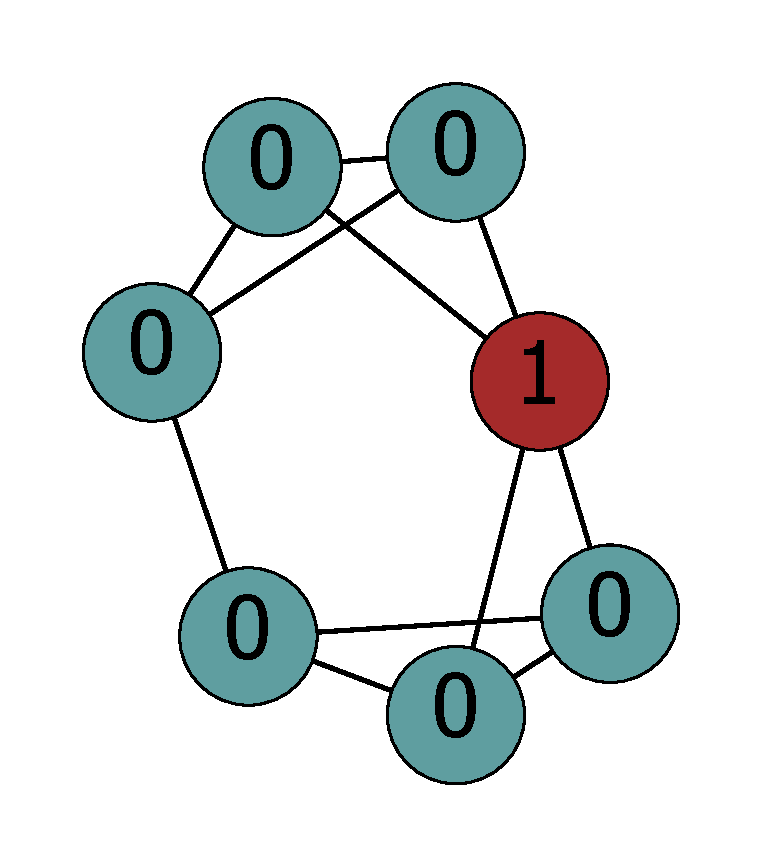
\includegraphics[scale=0.35]{pictures/010110010110101011010[0,0,0,0,0,0,1].pdf}
	\caption{The seed blocks.}
	\label{fig:seeds}
\end{figure}

Lemma \ref{SubdivideTwice} part (2) suggests a way to construct $G$ such that $(G,h)$ is not AT from smaller graphs.  Specifically, we have the following.
\begin{cor}\label{SubdivideConstructor}
	If $e$ is an edge in $G$ such that $(G,h)$ is not AT and $(G-e, h)$ is not AT, then $(G',h')$ is not AT where $(G',h')$ is formed from $(G,h)$ by subdividing $e$ twice and having $h'$ give zero on the two new vertices.
\end{cor}

Let $\B$ be the smallest collection of pairs $(G,h)$ containing the pairs in Figure \ref{fig:seeds} that is closed under the operation in Corollary \ref{SubdivideConstructor}.

\begin{conjecture}\label{ClassificationDegreeThreePlus}
	Let $G$ be a connected graph and $x \in V(G)$ a noncutvertex with $d_G(x) \ge 3$.  If $h(x) = 1$ and $h(v) = 0$ for all $v \in V(G-x)$, then $(G,h)$ is not AT if and only if
	$x$ is in a block $B$ such that $(B, h') \in \B$ with $h'(x) = 1$ and every other block of $G$ is complete or an odd cycle.
\end{conjecture}

\bibliographystyle{amsplain}
\bibliography{GraphColoring1}

\end{document}
